\chapter{Project Progress\label{ch:project_progress}}

The software design for each sprint is done ahead of the respective sprint.
This procedure goes along well with the Agile Manifesto which
encourages the design of a complex system in small incremental parts.


\section{Sprint 1: Alpha Version}

The existing architecture of \ac{AnSiAn} features individual threads for scheduling, 
downsampling, demodulation and audio output. The \texttt{De\-mo\-du\-la\-tor} thread demodulates 
quadrature samples by calling the \texttt{demodulate()} method on an instance of
\texttt{Demodulation}. \texttt{Demodulation} is an abstract class that is implemented by concrete 
demodulation methods such as \texttt{AM}, \texttt{FM} and \texttt{Morse}. 

\ac{AnSiAn} utilizes the EventBus library in order to pass demodulated Morse text
to the \ac{GUI}. Demodulated audio data is passed to the
\texttt{AudioSink} thread by enqueuing it into its input queue.
This mechanism is explained in more detail in \autoref{sec:cleanup.mem}.


In order to extend \ac{AnSiAn} with demodulation functionality for \ac{PSK31} and \ac{RDS}, 
the existing architecture needs to be extended. The extended architecture is
depicted in \autoref{fig:demod_text_eventbus} and explained in the following.

\begin{figure}
	\centering
	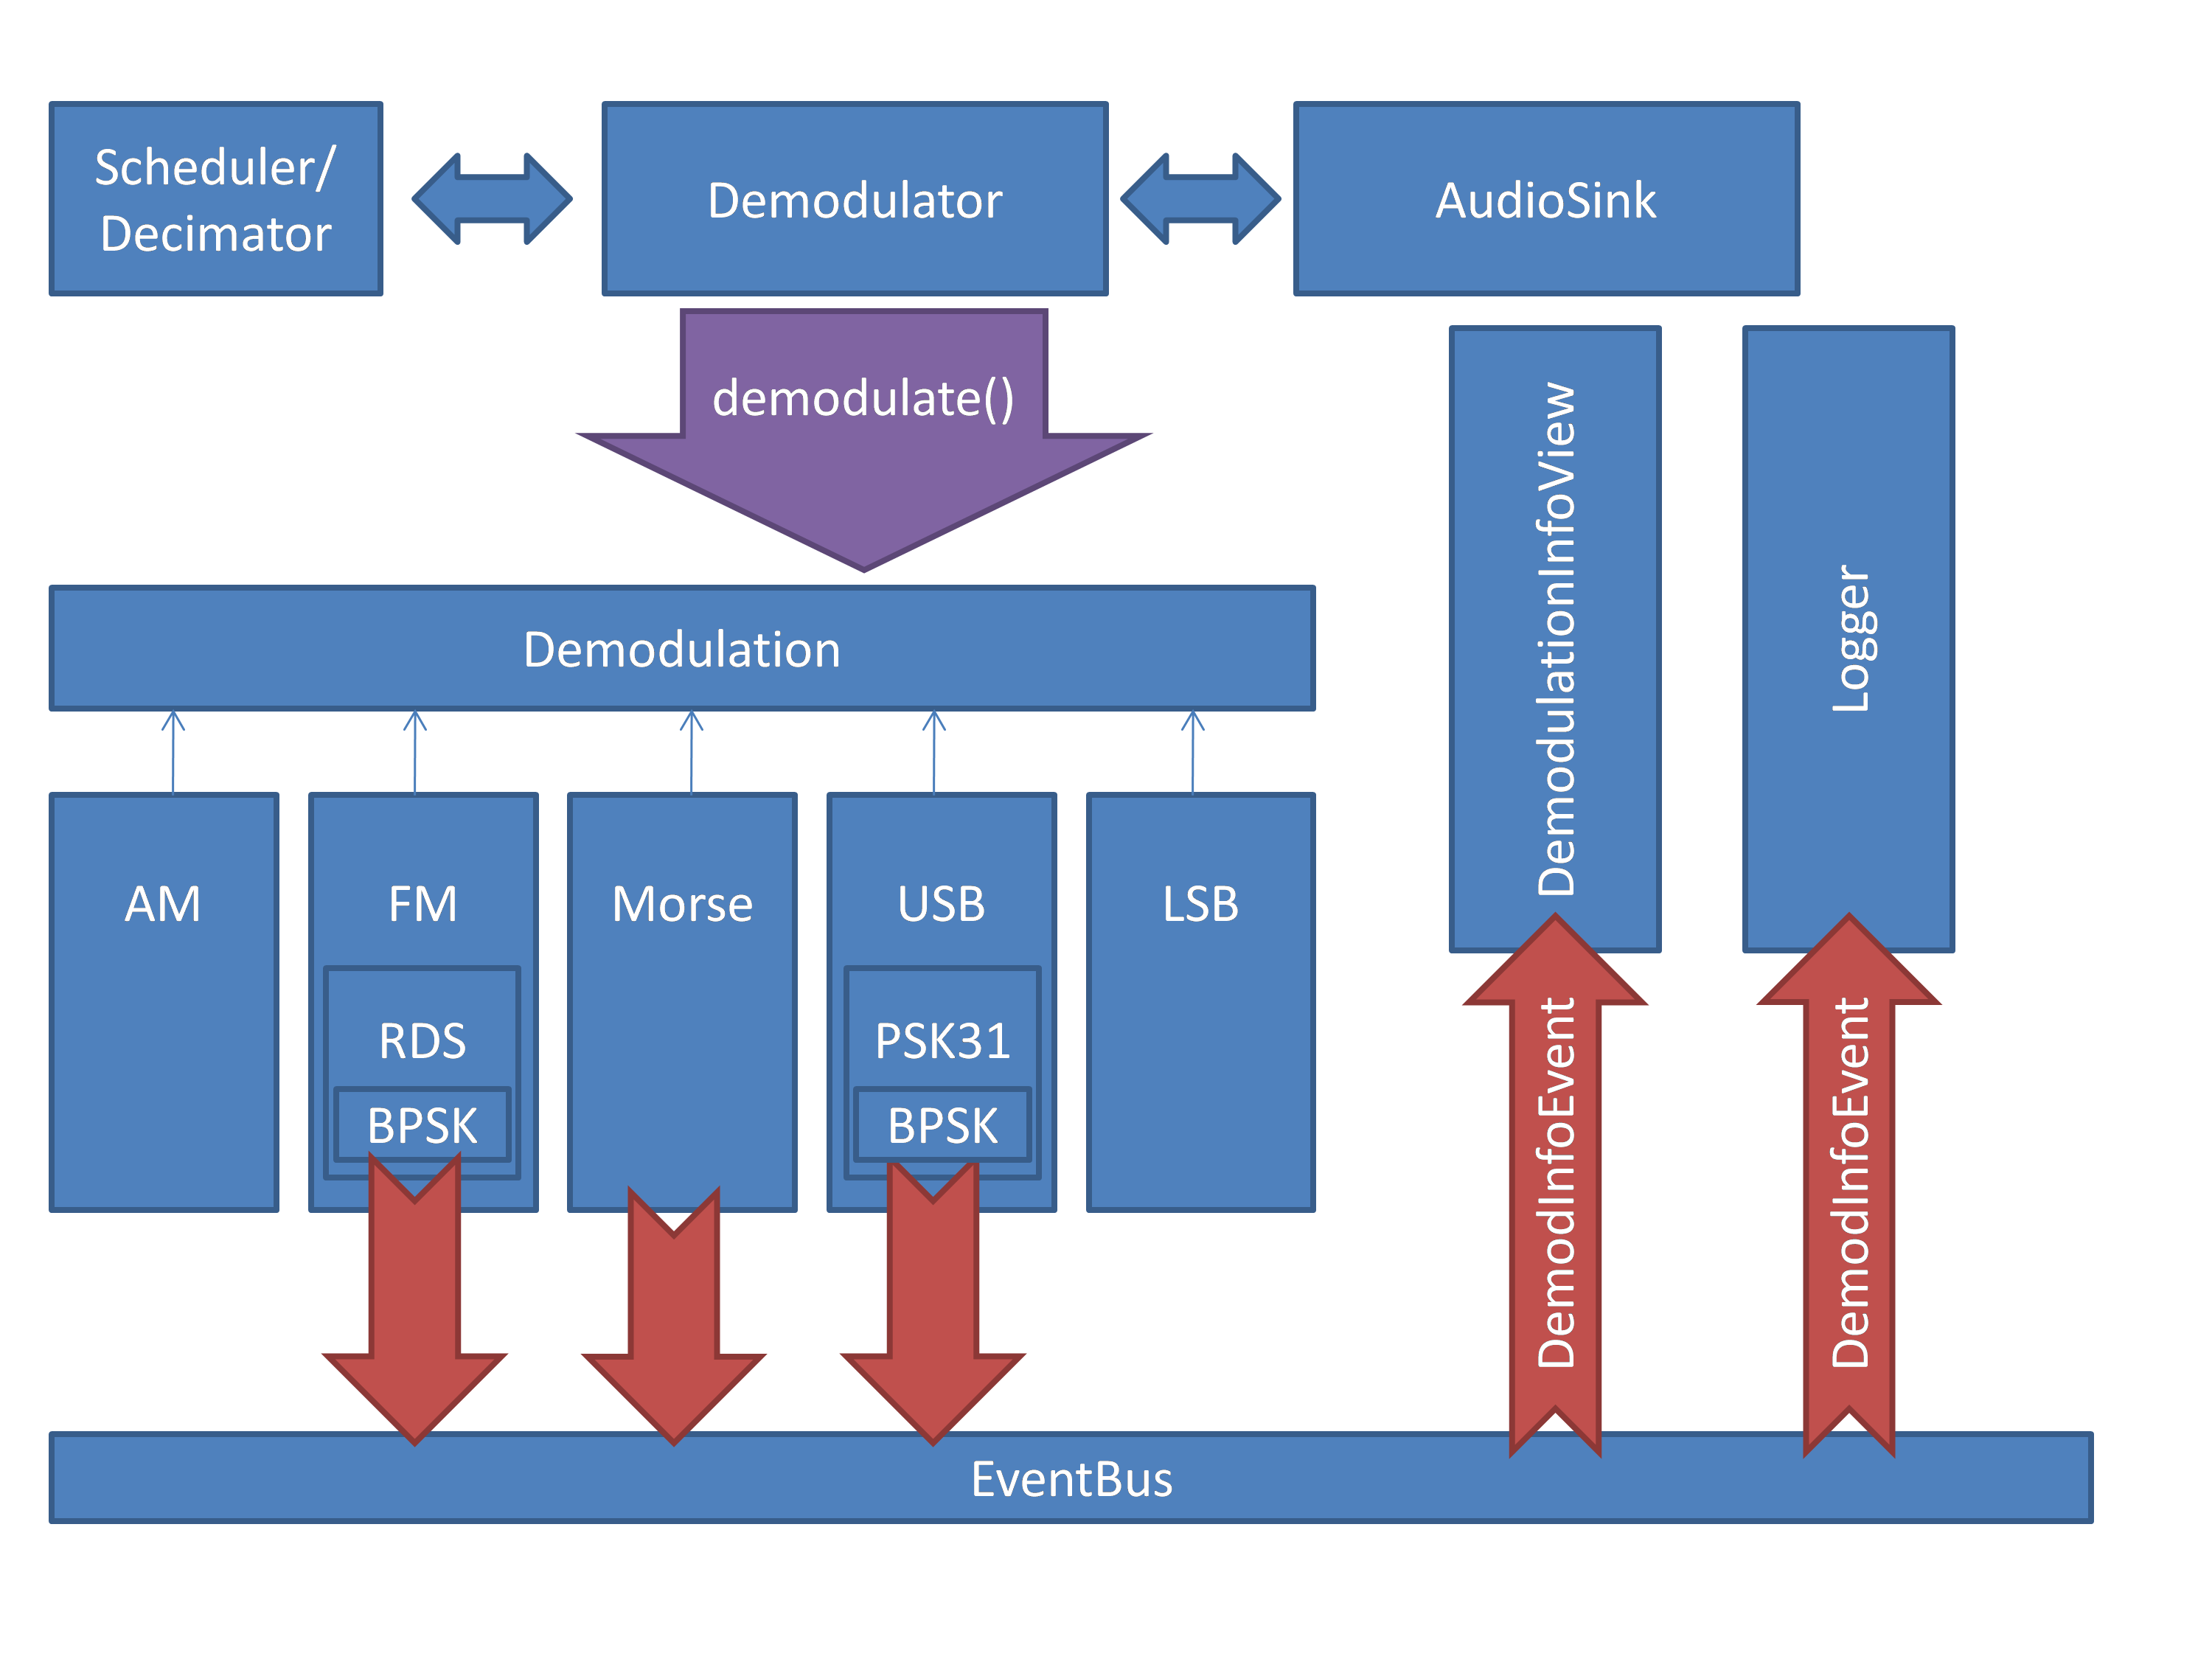
\includegraphics[width=1\linewidth]{gfx/demod_text_eventbus.png}
	\caption{Architecture of the extended demodulation logic and communication with the GUI}
	\label{fig:demod_text_eventbus}
\end{figure}

Two new classes \texttt{PSK31} and \texttt{RDS}, that inherit from
\texttt{Demodulation}, need to be implemented to represent the new demodulation 
mechanisms.

As \ac{PSK31} demodulation works on the envelope of the received signal
and \ac{AM} demodulation essentially performs envelope detection, \texttt{PSK31}
uses an instance of \texttt{AM} for envelope detection.

\ac{RDS} transmits metadata for \ac{FM} radio channels. It is therefore desirable for the 
\ac{RDS} demodulation mode to not only display this metadata, but to also play the 
\ac{FM}-modulated audio at the same time. The \texttt{RDS} class uses an
instance of \texttt{FM} for this purpose.

Like the existing architecture, the new architecture will use the EventBus
library to pass the demodulated text to the \ac{GUI}. The existing View
\texttt{MorseReceiveView} is refactored into a universal
\texttt{De\-mo\-du\-la\-tion\-In\-fo\-View} that displays the text output of any selected 
demodulator. Demodulators pass \texttt{DemodTextEvent}s and 
\texttt{DemodInfoEvent}s via the EventBus to the \texttt{De\-mo\-du\-la\-tion\-In\-fo\-View}, 
which contain demodulated text and further information (e.g. baud rates or raw 
dits and dahs) and are displayed in separate lines.

\section{Sprint 2: Beta Version}
\section{Sprint 3: Final Version}